\section*{Zielsetzung}
In diesem Versuch ist das Ziel die Funktionsweise eines Lock-In Verstärkers zu untersuchen und verstehen.

\section{Theorie}
Im Allgemeinen ist ein Lock-In Verstärke aus einem Bandpassfilter, einem Phasenverschieber, einem Mischer und einem Tiefpassfilter. Der schematische 
Aufbau ist in der \autoref{fig:1} dargestellt.

\begin{figure}[H]
    \centering
    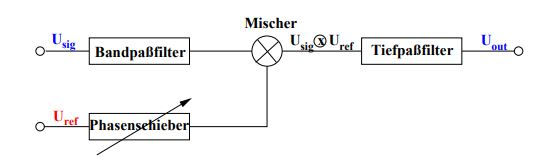
\includegraphics{Picture/0.jpg}
    \caption{Aufbau eines Lock-In-Verstärkers %\cite{}
    }
    \label{fig:1}
\end{figure}

\noindent
Der Bandpassfilter filtert stark hoch- und niederfrequente Freuquenzen des Nutzsignals $U_\text{sig}$ raus. Mithilfe des Phasenverschiebers ist es möglich, wie es der Name schon suggeriert, die Phase des Referenzsignals $U_\text{ref}$ zum Nutzsignals $U_\text{sig}$ zu verschieben. Im Mischer werden die beiden Signale miteinander multipliziert. Hinter dem Mischer ist ein Tiefpass ($\tau = RC ≫ 1/\omega_0$) verschaltet,  der das Mischsignal  $U_\text{sig} \times U_\text{ref}$ integriert. Durch solch einen Aufbau sind Güten in der Größenordnung $Q=10^6$ erreichbar, während eine reine Bandpass-Schaltung nur Güten in einem Bereich von $Q=10^3$ erreicht. \par
Das Referenzsignal $U_\text{ref}$ ist im Allgemeinen eine Rechteckspannung und kann durch eine Fourier-Reihe Form 
\begin{equation}
    U_\text{ref} = \frac{4}{\pi}(\sin(\omega \cdot t) + \frac{1}{3}\sin(3\omega \cdot t) +  \frac{1}{5}\sin(5\omega \cdot t) + ...)
    \label{eqn:uref}
\end{equation}

\noindent
und das Nutzsignal kann als Sinusspannung der Form 

\begin{equation}
    U_\text{sig} = U_0 \cdot \sin(\omega \cdot t)
    \label{eqn:usig}
\end{equation}
\noindent
genähert werden. Daraus ergibt sich die Multiplikation zu der Form 
\begin{equation}
    U_\text{sig} \times U_\text{ref} = \frac{2}{\pi} \cdot U_0(1 - \frac{2}{3}\cos(2\omega \cdot t)  -  \frac{2}{15}\cos(4\omega \cdot t) - \frac{2}{35}\cos(6\omega \cdot t)...) \, .
    \label{eqn:urefsig}
\end{equation}

\noindent
Durch den Tiefpassfilter werden die Oberwellen des Signals, welches durch die Vermischung entstanden ist, rausgefiltert. Somit ist das Ausgangssignal
propotional zur Nutzspannung. Dies wird beschrieben durch
\begin{equation}
    U_\text{out} = \frac{2}{\pi} U_0 \cdot \cos(\phi) \, ,
    \label{eqn:uout2}
\end{equation}

\noindent
wobei $\phi$ die Phasendifferenz zwischen den beiden Signalen beschreibt. Die Ausgangsspannung wird also für eine Phase von $\phi=0$ maximal.